\subsection{Building the C runtime system}

The C runtime system contains some basic functionalities to run the generated models. The so called 
runtime is common for all C projects. The requirements for several projects may differ depending on the 
functionality of the model or the resources of the different platforms. Therefore the runtime is 
configurable in terms of message queue size, frequency and memory alignment. The configuration file 
\textit{etRuntimeConfig.h} is located in \textit{src/config}.

After changing the configuration, the runtime must be built.

Open the properties of the \textit{org.eclipse.runtime.c} project and select \textit{C/C++ 
Build->Settings->Tool Settings} and select \textit{Includes}.

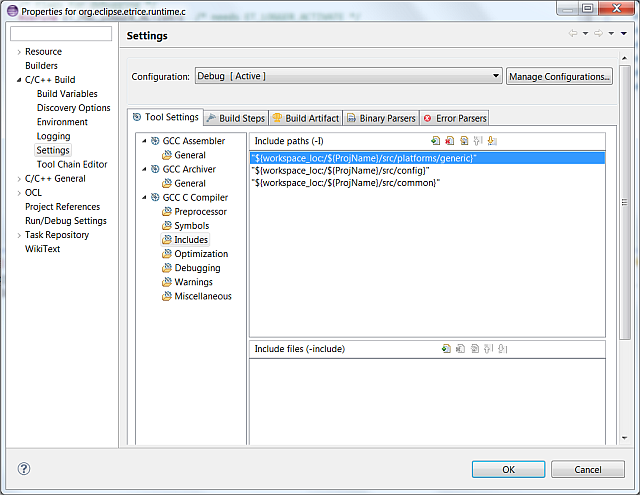
\includegraphics{images/014-SetupWorkspaceC08.png}
% !images/014-SetupWorkspaceC08.png!

Verify the include paths

\begin{itemize}
\item \textit{src/config}
\item \textit{src/common}
\item \textit{src/platforms/generic}
\end{itemize}

Within the Setting dialog select the tab \textit{Build Artefact} and select \textit{Static Library}

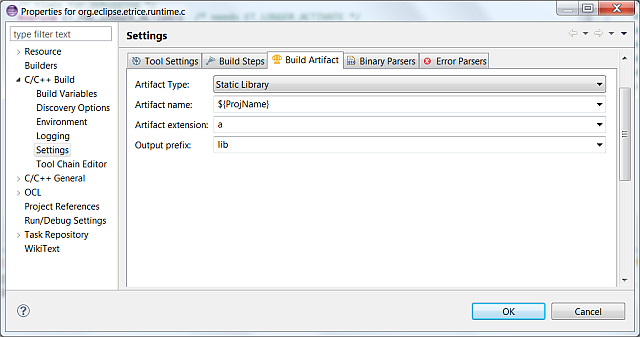
\includegraphics{images/014-SetupWorkspaceC09.png}
% !images/014-SetupWorkspaceC09.png!

Build the runtime by clicking

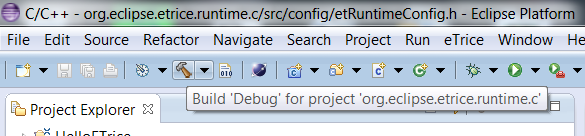
\includegraphics{images/014-SetupWorkspaceC10.png}
% !images/014-SetupWorkspaceC10.png!

The runtime library should be created.

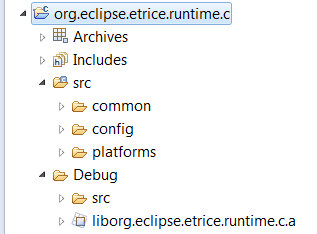
\includegraphics{images/014-SetupWorkspaceC11.png}
% !images/014-SetupWorkspaceC11.png!

For the tutorials one runtime library should be sufficient. For embedded projects it might be necessary to 
build project specific runtime libraries. In this case a separate project for the runtime should be 
created. Symbolic links to the sources might be used to avoid duplicate files. Just the configuration file 
must be duplicated. A specific library file must exist within the project. Such specific runtime libraries 
might be referenced from several applications.     
